\begin{frame}
    \centering
    \begin{figure}[H]
        \includegraphics[keepaspectratio, width=0.7\paperwidth, height=\paperheight]{\thelogo}
    \end{figure}
    Informatik: Programmieren\\
    \textbf{Feedback zu Übungen} \emoji{nerd-face}
\end{frame}

% default settings for listings
\lstset{style=python, basicstyle=\scriptsize\ttfamily,escapechar=!}

\begin{frame}[fragile]{Nützliche Shortcuts}

\begin{table}[H]
\scriptsize
\begin{tabular}{c|c|c}
\textbf{Aktion}&\textbf{Windows}&\textbf{MacOS}\\\midrule\midrule
Ausschneiden &\keys{\ctrl + X}& \keys{\cmd + X}\\\midrule
Kopieren &\keys{\ctrl + C}& \keys{\cmd + C}\\\midrule
Einfügen &\keys{\ctrl + V}& \keys{\cmd + V}\\\midrule
Suchen &\keys{\ctrl + F}& \keys{\cmd + F}\\\midrule
Datei speichern &\keys{\ctrl + S}& \keys{\cmd + S}\\\midrule
Rückgängig (``undo'') &\keys{\ctrl + Z}& \keys{\cmd + Z}\\\midrule
Vorwärts (``redo'') &\keys{\ctrl +\shift + Z}& \keys{\cmd + \shift + Z}\\\midrule
Cursor bewegen &\keys{\arrowkeyright}, \keys{\arrowkeyleft} & \keys{\arrowkeyright}, \keys{\arrowkeyleft}\\\midrule
Cursor bewegen (Wörter)\footnote{kann auch mit \keys{\shift} oder \keys{\del} kombiniert werden} &\keys{\ctrl+\arrowkeyright}, \keys{\ctrl+\arrowkeyleft} & \keys{\Alt+\arrowkeyright}, \keys{\Alt+\arrowkeyleft} \\\midrule
Einrücken & \keys{\tabwin}& \keys{\tab}\\\midrule
Ausrücken & \keys{\shift + \tabwin}& \keys{\shift + \tab}
\end{tabular}
\end{table}
\end{frame}


\begin{frame}[fragile]{Nützliche Shortcuts}

\begin{table}[H]
\scriptsize
\begin{tabular}{p{3.5cm}|c|c}
\textbf{Aktion}&\textbf{Windows}&\textbf{MacOS}\\\midrule\midrule
Fenster wechseln & \keys{\ctrl + \tabwin} & \keys{\cmd + \tab}\\\midrule
Browser: Tab wechseln & \keys{\ctrl + (\shift) + \tabwin}, \keys{\ctrl + zahl} & \keys{\cmd + (\shift) + \tab} \keys{\cmd + zahl}\\\midrule
Browser: Tab schliessen & \keys{\ctrl + W} & \keys{\cmd + W}\\\midrule
Browser: Neuen Tab öffnen & \keys{\ctrl + T} & \keys{\cmd + T} \\\midrule
Browser: Geschlossenen Tab wieder öffnen & \keys{\ctrl + \shift + T} & \keys{\ctrl + \shift + T}\\
\end{tabular}
\end{table}
\end{frame}

\begin{frame}[fragile]{Lektion 01: \lstinline|repeat|}
Welcher Code ist Ihnen lieber?

\begin{minipage}[t]{.45\textwidth}
    \begin{lstlisting}
from gturtle import*
makeTurtle()

repeat 1:
    forward(25)
    right(90)
    forward(25)
    left(90)
    forward(25)
    right(90)
    forward(25)
    left(90)
    forward(25)
    right(90)
    forward(25)
    left(90)
    # ...
\end{lstlisting}
\end{minipage}
\begin{minipage}[t]{.45\textwidth}
    \begin{lstlisting}
from gturtle import*
makeTurtle()

repeat 6 :
    fd(25)
    right(90)
    fd(25)
    left(90)
\end{lstlisting}
\end{minipage}
\end{frame}

\begin{frame}[fragile]{Lektion 01}{Was fehlt?}
\begin{lstlisting}
repeat 6 :
    fd(25)
    right(90)
    fd(25)
    left(90)
\end{lstlisting}
\end{frame}

\begin{frame}[fragile]{Lektion 01}{Was macht die letzte Zeile?}
\begin{lstlisting}
from gturtle import*
makeTurtle()
!\tikzmark{to}!
repeat 6 :
    fd(25)
    right(90)
    fd(25)
    left(90)
    
hide!\tikzmark{from}!Turtle()
\end{lstlisting}

\only<2->{
$\rightarrow$ Muss am richtigen Ort stehen!
\begin{tikzpicture}[overlay,remember picture]
\draw[red,-stealth] (from.north) to[bend right] (to);
\end{tikzpicture}}

\end{frame}

\begin{frame}[fragile]{Lektion 01: Stil}{Wo würden Sie neue Zeilen (=Zeilenumbrüche) machen?}
\begin{lstlisting}
from gturtle import*

makeTurtle()

repeat 6 :

    fd(25)
    
    right(90)
    
    fd(25)
    
    left(90)
    
\end{lstlisting}

\end{frame}



\begin{frame}[fragile]{Lektion 08}
\tib{Aufgabe 3.38} (Reiskörner): Was könnte hier besser gemacht werden?
\begin{lstlisting}
def summe(anzahl, zahl):
    resultat = 0
    repeat anzahl:
        print(zahl, resultat)
        resultat += zahl
        zahl*= 2
    print(resultat)
    
summe(63, 1)
\end{lstlisting}
\begin{itemize}
    \item Zeile 1: sind \pythoninline{resultat} und \pythoninline{zahl} gute Variablennamen?
    \item Zeile 2: weshalb \pythoninline{resultat=0}?
\end{itemize}
\end{frame}

\begin{frame}[fragile]{Lektion 09}
\tib{Aufgabe 3.40} (Wort $10\cdot 10$ mal drucken): Was könnte hier besser gemacht werden?
\begin{lstlisting}
from gturtle import*

makeTurtle()
def druckewort(anzahl):
    wort = input("Welche Zahl?")
    repeat(anzahl):
        print(wort*10)
        
druckewort(10)
\end{lstlisting}
\begin{itemize}
    \item Zeilen 1-3: Weshalb \pythoninline{from gturtle import*} und \pythoninline{makeTurtle()}?
    \item Zeile 4: Weshalb \pythoninline{def}?
    \item Zeile 5: Weshalb \pythoninline{input("Welche Zahl")}?
\end{itemize}
\end{frame}


\begin{frame}[fragile]{Lektion 10}
\tib{Aufgabe 4.11}: Was könnte hier besser gemacht werden?\\[-.5cm]
\begin{minipage}[t]{.49\textwidth}
    \begin{lstlisting}
from gturtle import*
def vieleck(ecken,seite,farbe):
    setPenColor(farbe)
    repeat ecken:
        forward(seite)
        right(360/ecken)
def vieleck_sicher(zahl):
    if zahl ==1:
        vieleck(4,50,"red")
    if zahl ==2:
        vieleck(3,50,"green")
    
        
    if zahl ==3:
        vieleck(6,50,"blue")
        
    else:
        print("Nur 1/2/3 gehen")

makeTurtle()
zahl =input("Zahl 1-10")
vieleck_sicher(zahl)
\end{lstlisting}
\end{minipage}
\begin{minipage}[t]{.49\textwidth}
    \begin{lstlisting}
from gturtle import *

def vieleck(ecken, seite, farbe):
    setPenColor(farbe)
    repeat ecken:
        forward(seite)
        right(360/ecken)
        
def vieleck_sicher(zahl):
    if zahl==1:
        vieleck(4, 50, "red")
    if zahl==2:
        vieleck(3, 50, "green")
    if zahl==3:
        vieleck(6, 50, "blue")
    else:
        print("Nur 1/2/3 gehen")

makeTurtle()
zahl=input("Zahl 1-10")
vieleck_sicher(zahl)
\end{lstlisting}
\end{minipage}
\begin{minipage}[c]{.45\textwidth}
    \begin{itemize}
        \item Finde die 10 Unterschiede...
    \end{itemize}
\end{minipage}
\begin{minipage}[c]{.48\textwidth}
    \begin{figure}[H]
    \centering
    
\includegraphics[keepaspectratio, width=.25\paperwidth, height=\paperheight]{GrundlagenInfo/00_Programmieren/Figures/prog-make_it_nice.jpeg}
    \end{figure}
\end{minipage}
\end{frame}

\begin{frame}[fragile]{Lektion 10}
\tib{Aufgabe 4.11}: Was könnte hier besser gemacht werden?\\[-.5cm]
\begin{minipage}[t]{.45\textwidth}
    \begin{lstlisting}
from gturtle import *

def vieleck(ecken, seite, farbe):
    setPenColor(farbe)
    repeat ecken:
        forward(seite)
        right(360/ecken)
        
def vieleck_sicher(zahl):
    if zahl==1:
        vieleck(4,50, "red")
    if zahl==2:
        vieleck(3,50, "green")
    if zahl==3:
        vieleck(6,50, "blue")
    else:
        print("Nur 1/2/3 gehen")

makeTurtle()
zahl=input("Zahl 1-10")
vieleck_sicher(zahl)
\end{lstlisting}
\end{minipage}
\begin{minipage}[t]{.45\textwidth}
    \begin{lstlisting}
from gturtle import *

def vieleck(ecken, farbe):
    setPenColor(farbe)
    repeat ecken:
        forward(50)
        right(360/ecken)
        
def vieleck_sicher(zahl):
    if zahl==1:
        vieleck(4, "red")
    if zahl==2:
        vieleck(3, "green")
    if zahl==3:
        vieleck(6, "blue")
    else:
        print("Nur 1/2/3 gehen")

makeTurtle()
zahl=input("Zahl 1-10")
vieleck_sicher(zahl)
\end{lstlisting}
\end{minipage}
\begin{minipage}[c]{.3\textwidth}
    \begin{figure}[H]
    \centering
    
\includegraphics[keepaspectratio, width=.25\paperwidth, height=\paperheight]{GrundlagenInfo/00_Programmieren/Figures/prog-make_it_nice.jpeg}
    \end{figure}
\end{minipage}
\begin{minipage}[c]{.66\textwidth}
    \begin{itemize}
        \item ... \& make it simple!
        \item Ein Parameter, der immer den gleichen Wert annimmt, kann als Konstante geschrieben werden
    \end{itemize}
\end{minipage}
\end{frame}


\begin{frame}[fragile]{Lektion 10}
\tib{Aufgabe 4.11}: Was könnte hier besser gemacht werden?\\[-.5cm]
\begin{minipage}[t]{.45\textwidth}
    \begin{lstlisting}
from gturtle import *

def vieleck(ecken, seite, farbe):
        
def vieleck_sicher(zahl):
    if zahl==1:
        setPenColor("red")
        repeat 4:
            forward(50)
            right(360/4)
    if zahl==2:
        setPenColor("red")
        repeat 3:
            forward(50)
            right(360/3)
    if zahl==3:
        setPenColor("green")
        repeat 6:
            forward(50)
            right(360/6)
    else:
        print("Nur 1/2/3 gehen")

makeTurtle()
zahl=input("Zahl 1-10")
vieleck_sicher(zahl)
\end{lstlisting}
\end{minipage}
\begin{minipage}[t]{.45\textwidth}
    \begin{lstlisting}
from gturtle import *

def vieleck(ecken, farbe):
    setPenColor(farbe)
    repeat ecken:
        forward(50)
        right(360/ecken)
        
def vieleck_sicher(zahl):
    if zahl==1:
        vieleck(4, "red")
    if zahl==2:
        vieleck(3, "green")
    if zahl==3:
        vieleck(6, "blue")
    else:
        print("Nur 1/2/3 gehen")

makeTurtle()
zahl=input("Zahl 1-10")
vieleck_sicher(zahl)
\end{lstlisting}
\end{minipage}
\begin{minipage}[c]{.48\textwidth}
    \begin{itemize}
        \item Code \tib{modularisieren}
    \end{itemize}
\end{minipage}
\begin{minipage}[c]{.48\textwidth}
    \begin{figure}[H]
        \centering
        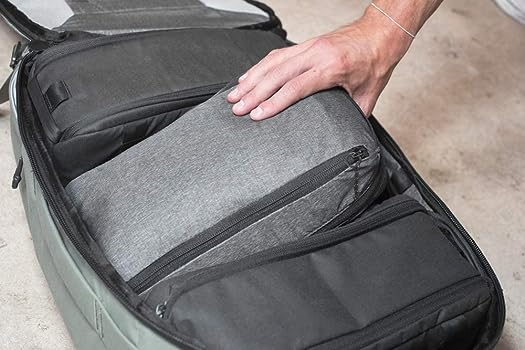
\includegraphics[keepaspectratio, width=.15\paperwidth]{GrundlagenInfo/00_Programmieren/Figures/prog-packing-cubes.jpg}
    \end{figure}
\end{minipage}
\end{frame}

\begin{frame}[fragile]{Lektion 10}
\tib{Aufgabe 4.11}: Was könnte hier besser gemacht werden?\\[-.5cm]
\begin{minipage}[t]{.49\textwidth}
    \begin{lstlisting}[basicstyle=\tiny\ttfamily]
from gturtle import*

def quadrat():
    repeat 4:
        forward(50)
        right(90)
        
def drehen():
    runden =input("Wie viele Runden?")
    repeat runden:
        repeat 360:
            setPenWidth(1)
            setPenColor("black")
            quadrat()
            delay(1)
            setPenWidth(10)
            setPenColor("white")
            quadrat()   
            right(1)
    
makeTurtle()
hideTurtle()
drehen()
\end{lstlisting}
\begin{figure}[H]
        \centering
        
\includegraphics[keepaspectratio, width=.13\paperwidth]{GrundlagenInfo/00_Programmieren/Figures/prog-comment.jpg}
    \end{figure}
\end{minipage}
\begin{minipage}[t]{.49\textwidth}
    \begin{lstlisting}[basicstyle=\tiny\ttfamily]
from gturtle import*

def quadrat():
    repeat 4:
        forward(50)
        right(90)
        
def drehen():
    runden =input("Wie viele Runden?")
    repeat runden:
        repeat 360:
            # quadrat malen
            setPenWidth(1)
            setPenColor("black")
            quadrat()
            delay(1) # 1 ms warten
            # quadrat auslöschen
            setPenWidth(10)
            setPenColor("white")
            quadrat()
            # nach rechts drehen
            right(1)
    
makeTurtle()
hideTurtle()
drehen()
\end{lstlisting}
\end{minipage}
\end{frame}

\begin{frame}{Code-Qualität \emoji{nerd-face}}{Zusammenfassung}
    Ein guter Code ist:
    \begin{itemize}
        \item möglichst \textbf{kurz und leserlich}
        \item \textbf{modular}, so dass man ihn einfach in Unterteile zerlegen kann
        \item schön und leserlich sowie \textbf{konsistent formatiert}
        \item gut dokumentiert mit \textbf{Kommentaren}
        \item \textbf{verständlich} und enthält \textbf{selbst-erklärende} Variablen- und Funktionen-Namen
    \end{itemize}
    \begin{figure}[H]
        \centering
        
\includegraphics[keepaspectratio, height=.15\paperheight]{GrundlagenInfo/00_Programmieren/Figures/prog-make_it_nice.jpeg}
        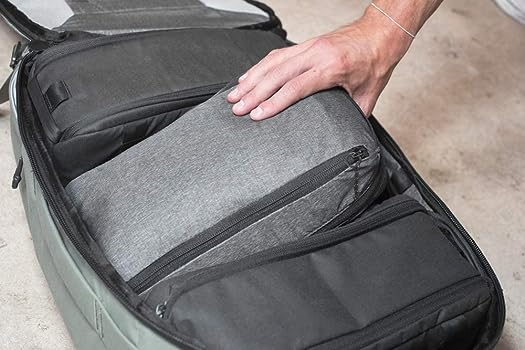
\includegraphics[keepaspectratio, height=.15\paperheight]{GrundlagenInfo/00_Programmieren/Figures/prog-packing-cubes.jpg}
        
\includegraphics[keepaspectratio, height=.15\paperheight]{GrundlagenInfo/00_Programmieren/Figures/prog-comment.jpg}
        
\includegraphics[keepaspectratio, height=.15\paperheight]{GrundlagenInfo/00_Programmieren/Figures/prog-confused.jpg}
    \end{figure}
\end{frame}




